
% \documentclass is book
\documentclass[12pt,twoside,letterpaper]{book}

\usepackage[utf8]{inputenc}
\usepackage{ifthen}   
\usepackage{comment}
\usepackage{tikz}
\usepackage{smartdiagram}
\usepackage{pstricks}
\usepackage{cite}
\usepackage{graphicx}
\graphicspath{\fig }
\newcommand\tab[1][1cm]{\hspace*{#1}}
\setlength{\parindent}{0pt}
\newcommand{\forceindent}{\leavevmode{\parindent=4em\indent}}
% Creative Commons
\usepackage[
   type={CC},
   modifier={by-nc-sa},
   version={4.0},
]{doclicense}
\newenvironment{myindentpar}[1]%
  {\begin{list}{}%
          {\setlength{\leftmargin}{#1}}%
          \item[]%
  }
  {\end{list}}
%------------------------tikz
\usetikzlibrary{shapes,arrows}
\tikzstyle{decision} = [diamond, draw, fill=blue!20, 
    text width=4em, text badly centered, node distance=2.25cm, inner sep=0pt]
\tikzstyle{block} = [rectangle, draw, fill=gray!20, 
    text width=10em, text centered, rounded corners, minimum height=3em]
\tikzstyle{line} = [draw, -latex']
\tikzstyle{cloud} = [draw, ellipse,fill=red!20, node distance=3cm,
    minimum height=2em]
%------------------------

% provide if-then-else operators

% --------------------------------------------------------------------------
% Global variables required in document formatting
% --------------------------------------------------------------------------
%
% BOOK MODE
%
\newboolean{bookmode}                  % boolean used to control book format
% Ensure that only one of the next two lines is active:
\setboolean{bookmode}{true}           % turn book mode on
%\setboolean{bookmode}{false}           % turn book mode off

%
% DRAFT MODE
%
\newboolean{draftmode}                  % boolean used to control draft-mode
% Ensure that only one of the next two lines is active:
%\setboolean{draftmode}{true}            % turn draft mode on
\setboolean{draftmode}{false}           % turn draft mode off
% --------------------------------------------------------------------------
%
% GENERAL AUTHOR, TITLE AND KEYWORDS
%
% Nombre del Estudiante
\newcommand{\scriptAuthor}{Steven Antonio Jiménez Bustamante}

% Título de la tesis
\newcommand{\scriptTitle}{Implementación de un sistema para la asistencia de pacientes mediante el robot Pepper} 

% Keywords
\newcommand{\scriptKeywords}{Visión por Computadora, ADAS, Aproximada}

% Descripción de la editorial
\newcommand{\boxeditorial}{%
}

% Para el PDF (cambiar si se desea otras cosas a lo indicado arriba
\newcommand{\pdfAuthor}{\scriptAuthor}
\newcommand{\pdfTitle}{\scriptTitle} 
\newcommand{\pdfKeywords}{\scriptKeywords}

% --------------------------------------------------------------------------

% include all packages and define all required general macros
%%%%%%%%%%%%%%%%%%%%%%%%%%%%%%%%%%%%%%%%%%%%%%%%%%%%%%%%%%%%%%%%%%%%%%%%%%%%%%%
% Author:  Pablo Alvarado
%
% Escuela de Electrónica
% Instituto Tecnológico de Costa Rica
%
% Phone:   +506 550 2106
% Fax:     +506 591 6629
% email:   palvarado@ietec.org
%
% $Id: macros.tex 1497 2010-08-09 17:04:26Z palvarado $
%
%%%%%%%%%%%%%%%%%%%%%%%%%%%%%%%%%%%%%%%%%%%%%%%%%%%%%%%%%%%%%%%%%%%%%%%%%%%%%%%

% Configuration of the exercises package, which is used to collect all
% problems and answers in the document.
\usepackage[exercisedelayed,answerdelayed,lastexercise]{exercise}
\renewcounter{Exercise}[chapter]
\renewcommand{\ExerciseName}{Problema}
\renewcommand{\theExercise}{\thechapter.\arabic{Exercise}}
\newcommand{\ExerciseLabel}{Exercise.\theExercise}
\renewcommand{\ExerciseHeader}%
{\textbf{\ExerciseName\ \theExercise.\ \ExerciseHeaderTitle\ }}
\renewcommand{\AnswerHeader}%
{\textbf{\ExerciseName\ \theExercise.\ }}


\usepackage{ifpdf}

% Command to change between draft or release mode:
\newcommand{\ifdraft}[2]{\ifthenelse{\boolean{draftmode}}{#1}{#2}}
% Command to change between draft or release mode:
\newcommand{\ifbook}[2]{\ifthenelse{\boolean{bookmode}}{#1}{#2}}

% include all required packages here
\usepackage[spanish,english]{babel}     % supports english, but default is 
                                        % spanish...
\newcommand*{\SelectSpanish}{%          % well, the last line indeed selects
  \hyphenrules{spanish}%                % english over spanish, but with this
  \languageshorthands{spanish}%         % command we turn it around.
  \captionsspanish                      % The reason: hyperref has some
  \datespanish                          % problems with the spanish babel,
}                                       % so we use some trick here so that it
\AtBeginDocument{\SelectSpanish}        % thinks it is english.

\usepackage{makeidx}                    % to create index file

\ifdraft{%
  %\usepackage[refpage]{nomencl}        % Use to easily administrate the list
 \usepackage{nomencl}                   % of symbols
}{%
 \usepackage{nomencl}
}
%\usepackage{times}                     % replace latex pk fonts with ps type I
                                        % don't forget to use dvips -D600 -Pcmz
                                        % to ensure Type I fonts!
\usepackage{amsmath}
\usepackage{amssymb,amstext}            % AMS-math and symbols package
\usepackage{mathrsfs}                   % Calygraphic fonts for transforms
\usepackage{array}                      % extensions to tabular environment
\usepackage{longtable}                  % supports extraordinary long tables
\usepackage{tabularx}                   % supports tables with fixed width
\usepackage{afterpage}                  % put something only after the page
\usepackage{multirow}                   % supports multiple row grouping in 
                                        % tables
\usepackage{multicol}                   % multiple columns environments
\usepackage{paralist}                   % a few enumeration settings


\usepackage{tikz}
\usetikzlibrary{shapes.geometric, arrows}

\usepackage[hang,%
            small,%
            bf]{caption}                % nicer figure captions
%\usepackage{sty/ftcap}                 % switch \abovecaptionskip and
%                                       % \belowcaptionskip for tables, in 
%                                       % order to avoid the caption to be
%                                       % too near to the table itself
% locally added packages
\usepackage{float}                      % really place figures "here" (H)
\usepackage{booktabs}                   % book type tabulars

% the own style with options depending on the draft mode
\ifdraft{%
\usepackage[todo]{sty/tecStyle}         % some command definitions
                                        % options [todo] todo-index
}{%
\usepackage{sty/tecStyle}               % some command definitions
                                        % options [todo] todo-index
}

%% fix the title for examples
\renewcommand{\examplelistname}{Índice de ejemplos}
\renewcommand{\examplename}{Ejemplo}


\usepackage{url}                        % allows linebreaks at certain
                                        % characters or combinations of 
                                        % characters for URLs

\usepackage[nottoc]{tocbibind}          % Fix the hyperrefs to TOC,TOF, etc.
                                        % and ensure that they appear all in 
                                        % the Table of Contents

\usepackage{color}                      % Support for colors
\definecolor{dkred}{rgb}{0.5,0,0}       %   dark red
\definecolor{dkgreen}{rgb}{0,0.3,0}     %   dark green
\definecolor{dkblue}{rgb}{0,0.0,0.5}    %   dark blue
\definecolor{dkgray}{gray}{0.4}         %   dark gray
\definecolor{dkmagenta}{rgb}{0.3,0.0,0.3} % dark magenta
\definecolor{ltyellow}{rgb}{1.0,1.0,0.7}  % light yellow

\newcommand{\bG}[1]{\textcolor{dkgreen}{\textbf{#1}}}
\newcommand{\bR}[1]{\textcolor{dkred}{\textbf{#1}}}
\newcommand{\bB}[1]{\textcolor{dkblue}{\textbf{#1}}}
\newcommand{\bM}[1]{\textcolor{dkmagenta}{\textbf{#1}}}
\newcommand{\bY}[1]{\textcolor{dkyellow}{\textbf{#1}}}
\newcommand{\bC}[1]{\textcolor{dkcyan}{\textbf{#1}}}

% For pdflatex
% - The hyperref package should always be loaded last, since it has to
%   overwrite some of the commands.
% - The package subfigure caused that the pagebackrefs and index refs were set
%   incorrectly.

\ifpdf
%
% final / draft document options
\usepackage[pdftex,final]{graphicx}     % for inserting pdf-graphics.
                                        % options final / draft
\ifdraft{%

\usepackage[pdftex,%
            pdftitle={\pdfTitle},%
            pdfauthor={\pdfAuthor},%
            pdfsubject={Notas de Clase},%
            pdfkeywords={\pdfKeywords},%
            naturalnames=true,
            linktocpage,
            hyperindex,
            colorlinks,
            urlcolor=dkred,          %\href to external url
            filecolor=dkmagenta,     %\href to local file
            linkcolor=dkred,         %\ref and \pageref
            citecolor=dkgreen,       %\cite
            pagecolor=dkred,
            pagebackref,
            plainpages=false,
            pdfpagelabels,
            pdfpagemode=UseOutlines, % means use bookmarks (None,UseOutlines)
            % bookmarksopen=false,   % would show the whole hierarchy if true
            bookmarksnumbered=true,
            pdfpagelayout=OneColumn, % SinglePage,OneColumn,TwoColumnLeft,...
            pdfview=FitH, % FitB,FitBH,FitBV,Fit,FitH,FitV
            pdfstartview=FitH, % FitB,FitBH,FitBV,Fit,FitH,FitV
            ]{hyperref}
}{%
\usepackage[pdftex,%
            pdftitle={\pdfTitle},%
            pdfauthor={\pdfAuthor},%
            pdfsubject={Notas de clase},%
            pdfkeywords={\pdfKeywords},%
            naturalnames=true,
            linktocpage,hyperindex,
            colorlinks,
            urlcolor=dkred,          %\href to external url
            filecolor=dkmagenta,     %\href to local file
            linkcolor=dkred,         %\ref and \pageref
            citecolor=dkgreen,       %\cite
            pagecolor=dkred,
            % pagebackref,           % only in draft modus should this be on.
            plainpages=false,
            pdfpagelabels,
            pdfpagemode=UseOutlines, % means use bookmarks (None,UseOutlines)
            % bookmarksopen=false,   % open the whole hierarchy if true!
            bookmarksnumbered=true,
            pdfpagelayout=OneColumn, % SinglePage,OneColumn,TwoColumnLeft,...
            pdfview=FitH, % FitB,FitBH,FitBV,Fit,FitH,FitV
            pdfstartview=FitH, % FitB,FitBH,FitBV,Fit,FitH,FitV
            ]{hyperref}
}




%
% Ensure that the links of the images point to the top of the images and not
% to the caption
%
\usepackage[figure]{hypcap}

% %
% % Ensure that pdfLaTeX do the same spacing as LaTeX
% %
\pdfadjustspacing=1 
% %
\else   % i.e. if not pdf

\usepackage[active]{srcltx}             % insert links into the dvi to jump
\usepackage[dvips,final]{graphicx}      % for inserting eps-graphics.
                                        % options final / draft
                                        % into the sources directly.
\ifdraft{%
\usepackage[ps2pdf,%
            pdftitle={\pdfTitle}%
            pdfauthor={\pdfAuthor},%
            pdfsubject={Notas de clase},%
            pdfkeywords={\pdfKeywords},%
            % plainpages=false,
            linktocpage,
            hyperindex,
            pagebackref,
            % pdfpagelabels,
            pdfpagemode=UseOutlines,
            pdfstartview=FitH]{hyperref}
}{%
\usepackage[ps2pdf,%
            pdftitle={\pdfTitle}%
            pdfauthor={\pdfAuthor},%
            pdfsubject={Notas de clase},%
            pdfkeywords={\pdfKeywords},%
            % plainpages=false,
            linktocpage,
            hyperindex,
            % pagebackref,
            % pdfpagelabels,
            pdfpagemode=UseOutlines,
            pdfstartview=FitH]{hyperref}
}

%\usepackage[ps2pdf]{hyperref}

\fi  % end of if pdf or not

\usepackage{sty/algorithmic}            % algorithmic environment


\usepackage{rotating}                   % allow block rotation


%%%%%%%%%%%%%%%%%%%%%%%%%%%%%%%%%%%%%%%%%%%%%%%%%%%%%%%%%%%%%%%%%%%%%%%%%%%%%%%

%\sloppy

%
% Some own font definitions
%
\DeclareMathAlphabet{\mathpzc}{OT1}{pzc}{m}{it}
\DeclareMathAlphabet{\mathpss}{OT1}{cmss}{m}{sl}

%
% page layout
%

\usepackage{vmargin}
\setpapersize{USletter}

% For letter-paper printing
\setmarginsrb{33mm}{8mm}{23mm}{7mm}{15pt}{15pt}{7mm}{12mm}
%\setlength{\headheight}{15pt}         % fancy headers wanted this

%
% Fraction of Float Object / Text
%

\renewcommand{\topfraction}{0.95}       % how much of top of page should be 
                                        % allowed to be float object?
\renewcommand{\bottomfraction}{0.95}    % how much of bottom of page should be
                                        % allowed to be float object?
\renewcommand{\textfraction}{0.05}      % how much of page must be text?

\usepackage{fancyhdr}                   % fancy page headers

\usepackage{lastpage}

%
% header and footer layout (needs package fancyhdr)
%
\newcommand{\copyrightfooter}{\tiny{\copyright 2005-2010 --- P.~Alvarado %
    \qquad Uso exclusivo ITCR}}
%
\newcommand{\draftfoot}%
  {\ifdraft{\textcolor{dkblue}{\tiny\textsl{Borrador: \today}}{}}
           {}
}

\pagestyle{fancy}
\renewcommand{\chaptermark}[1]{\markboth{{\small
    \thechapter\hspace*{1mm}#1}}{}}
\renewcommand{\sectionmark}[1]{\markright{{\small
    \thesection\hspace*{1mm}#1}}{}}
\lhead[{\small\textbf\thepage}]{\fancyplain{}%
        {{\slshape \small\nouppercase{\leftmark}}}}
\chead[]{}
\rhead[\fancyplain{}%
        {{\slshape \small\nouppercase{\rightmark}}}]{{\small\textbf\thepage}}
\lfoot[]{\draftfoot}
\ifbook{%
  \cfoot[]{}
}{
  \cfoot[\copyrightfooter]{\copyrightfooter}
}
\rfoot[\draftfoot]{}
\renewcommand{\headrulewidth}{0.5pt}
\renewcommand{\footrulewidth}{0pt}

%
% Caption style for tables
% Requires the packages caption2 and ftcap
% (caption2 required this, but is obsolete now:)
%
%\newcaptionstyle{tablecaptionstyle}{%
%  \renewcommand\captionlabelfont{\normalsize\bf}
%  \renewcommand\captionfont{\normalsize}
%  \usecaptionstyle{hang}%
%}

% For caption v3:
\captionsetup[table]{position=top,format=hang,textfont={normalsize},labelfont={normalsize,bf}}

\newcommand{\tablecaption}[2][foo]{%
  \ifthenelse{\equal{#1}{foo}}{%
    %\captionstyle{tablecaptionstyle}%
    \caption{#2}%
  }
  {%
    %\captionstyle{tablecaptionstyle}%
    \caption[#1]{#2}%
  }
}
\addto\extrasspanish{\renewcommand{\tablename}{Tabla}}
\addto\extrasspanish{\renewcommand{\listtablename}{\'Indice de tablas}}

%
% paragraph layout
%
\renewcommand{\baselinestretch}{1.1}    % line spacing
\parindent0em                           % indentation width of first line
\parskip1.3ex                           % space between paragraphs

%
% document consists of
% chapter - section - subsection - subsubsection - paragraph - subparagraph
%
\setcounter{secnumdepth}{2}             % depth of section numbering
\setcounter{tocdepth}{2}                % depth of table of contents

%
% prepares index from entries like \index{word} or \index{group!word}.
% don't forget to call "makeindex filename" for final index generation.
%
\makeindex                            %% for package makeidx.sty
%\newindex{default}{idx}{ind}{Index}  %% for package index.sty

\newcommand{\octave}{GNU/Octave}


%
% prepares notation or nomenclature 
%
%\makeglossary
\makenomenclature

%%% Local Variables: 
%%% mode: latex
%%% TeX-master: "main"
%%% End: 


% allow equations to be splitted (breaked) into several pages
\allowdisplaybreaks[3]

% --------------------------------------------------------------------------
\begin{document}
  % where to look for graphics
  \graphicspath{{./}{./fig/}}

  \pagenumbering{alph}
  % fix some terms not activated due to the bug of hyperref with spanish.
  \renewcommand{\tablename}{Tabla}
  \renewcommand{\listtablename}{\'Indice de tablas}
  \renewcommand{\examplesolution}{Solución}
  \pagestyle{empty}

  %% ---------------------------------------------------------------------------
%% titlepage.tex
%%
%% Title page
%%
%% $Id: titlepage.tex 1452 2010-07-07 00:55:16Z palvarado $
%% ---------------------------------------------------------------------------

\thispagestyle{empty} 

\begin{center}


Instituto Tecnológico de Costa Rica \\
Área Académica de Ingeniería Mecatrónica

\vspace{10pt}

%Programa de Licenciatura en Ingeniería Mecatrónica


\par\vspace{25mm}


\includegraphics[width=100mm]{fig/MarcaTECRGB.png}

\par\vspace*{\fill}

{\large\bf{\scriptTitle}}

\par\vspace*{\fill}

para optar por el título de \\
{\sf Ingeniero en Mecatrónica} \\

\vspace{8pt}

con el grado acad\'emico de \\
{\sf Licenciatura} \\

\par\vspace{25mm}

\scriptAuthor

\vspace*{\fill}

{Cartago, \today}

\end{center}
\newpage 
\cleardoublepage 


%%% Local Variables: 
%%% mode: latex
%%% TeX-master: "main"
%%% End: 
                                 % Titlepage
  \thispagestyle{empty}

\rule{10mm}{0pt}

\vfill

Declaro que el presente informe Proyecto de Graduación ha sido realizado enteramente
por mi persona, utilizando y aplicando literatura referente al tema e
introduciendo conocimientos propios.

En los casos en que he utilizado bibliografía he procedido a indicar las
fuentes mediante las respectivas citas bibliográficas.  En consecuencia,
asumo la responsabilidad total por el trabajo de graduación realizado y por
el contenido del correspondiente informe final.



\vspace*{8mm}

\begin{flushright}
  \scriptAuthor\par
  Cartago, \today\par
  Céd: 1-1579-0679
\end{flushright}

\vspace*{8mm}

\begin{center}
  \doclicenseThis
\end{center}

\cleardoublepage

%%% Local Variables: 
%%% mode: latex
%%% TeX-master: "main"
%%% End: 

  \thispagestyle{empty}

%%
%% Indique los nombres de los lectores y asesor
\newcommand{\lectorI }{M.Sc. Ing. \,Gabriela Ortiz León     }
\newcommand{\lectorII}{M.Sc. Ing. \,Sergio Arriola Valverde }
\newcommand{\director}{M.Sc. Ing. \,Yeiner Arias Esquivel  }
%% Revise además que 


\begin{center}
  \begin{tabular}{c}
    Tecnológico de Costa Rica \\
    Área Académica de Ingeniería Mecatrónica \\
    Proyecto de Graduación \\
    Tribunal Evaluador
  \end{tabular}
\end{center}

\vfill

Proyecto de Graduación defendido ante el presente Tribunal Evaluador como 
requisito para optar por el título de Ingeniero en Mecatrónica con el grado 
académico de Licenciatura, del Tecnológico de Costa Rica.  

\vfill

\vspace*{20mm}
\begin{center}
 Miembros del Tribunal
\end{center}
\vspace*{8mm}

\vfill

\begin{center}
  \begin{tabular}{ccc}
    \rule{70mm}{0.5pt} & \rule{15mm}{0pt} & \rule{70mm}{0.5pt} \\
    \lectorI && \lectorII \\
    Profesora Lectora && Profesor Lector
  \end{tabular}
  
  \vspace{10mm}

  \begin{tabular}{c}
    \rule{6cm}{0.5pt} \\
    \director \\
    Profesor Asesor
  \end{tabular}
\end{center}

\vfill


Los miembros de este Tribunal dan fe de que el presente trabajo de graduación
ha sido aprobado y cumple con las normas establecidas por Área Académica de
Ingeniería Mecatrónica.

\vfill

\begin{center}
  Cartago, 15 de enero de 2018\par
\end{center}

\cleardoublepage

%%% Local Variables: 
%%% mode: latex
%%% TeX-master: "main"
%%% End: 

  \thispagestyle{empty}

%%
%% Los nombres de lectores y asesor se definen en el archivo tribunal.tex
%%

\begin{center}
  \begin{tabular}{c}
    Tecnológico de Costa Rica \\
    Área Académica de Ingeniería Mecatrónica \\
    Proyecto de Graduación \\
    Tribunal Evaluador \\
    Acta de Evaluación
  \end{tabular}
\end{center}

\vfill

Proyecto de Graduación defendido ante el presente Tribunal Evaluador como 
requisito para optar por el título de Ingeniero en Mecatrónica con el grado 
académico de Licenciatura, del Tecnológico de Costa Rica.  

\vspace*{15mm}

\begin{center}
  Estudiante: Steven Antonio Jiménez Bustamante
\end{center}

\vfill

\begin{center}
  Nombre del Proyecto: \emph{Implementación de un sistema para la asistencia de pacientes mediante el robot Pepper}
\end{center}

\vspace*{20mm}
\begin{center}
 Miembros del Tribunal
\end{center}
\vspace*{8mm}

\vfill

\begin{center}
  \begin{tabular}{ccc}
    \rule{70mm}{0.5pt} & \rule{15mm}{0pt} & \rule{70mm}{0.5pt} \\
    \lectorI && \lectorII \\ %% Nombres definidos en tribunal.tex
    Profesora Lectora && Profesor Lector
  \end{tabular}
  
  \vspace{10mm}

  \begin{tabular}{c}
    \rule{6cm}{0.5pt} \\
    \director \\ %% Definido en tribunal.tex
    Profesor Asesor
  \end{tabular}
\end{center}

\vfill

Los miembros de este Tribunal dan fe de que el presente trabajo de graduación
ha sido aprobado y cumple con las normas establecidas por el Área Académica de
Ingeniería Mecatrónica.

\vfill

\begin{center}
  Nota final del Proyecto de Graduación: \rule{3cm}{0.5pt}
\end{center}
\vfill

\begin{center}
  Cartago, \today \par
\end{center}

\cleardoublepage

%%% Local Variables: 
%%% mode: latex
%%% TeX-master: "main"
%%% End: 

  \chapter*{Resumen}
\thispagestyle{empty}

Resumen Español

\bigskip

\textbf{Palabras clave: } \scriptKeywords Visión por computador, ROS, Robot Pepper, Faster R-CNN, Redes Neuronales Convolucionales, Deep Learning

\clearpage
\chapter*{Abstract}
\thispagestyle{empty}


Abstrac English

\bigskip

\textbf{Keywords:} Computer Vision, ADAS, Aproximate 

\cleardoublepage

%%% Local Variables: 
%%% mode: latex
%%% TeX-master: "main"
%%% End: 

  \vspace*{0.4\textheight}
{\hfill{\Large{\emph{a mis queridos padres}}}}

  %\chapter*{Agradecimientos}
\thispagestyle{empty}

El resultado de este trabajo no hubiese sido posible sin el apoyo de Oski, Luisito, Jota, Moncho, Piti, Manny, Marito, Ma, Pa, Ari, valentina JorgeKIT

\vspace*{1cm}

\scriptAuthor

Cartago, \today

\cleardoublepage

%%% Local Variables: 
%%% mode: latex
%%% TeX-master: "paMain"
%%% End: 


  %----------------------------------------------------------------------------
  \frontmatter
  %----------------------------------------------------------------------------
  \pagestyle{fancy}

  \pdfbookmark[1]{Indice General}{Indice General}

  \parskip0ex                           % space between paragraphs

  \tableofcontents                                      % Table of contents
  \listoffigures                                        % List of figures
  \listoftables                                         % List of tables

%\ifdraft{%
%  % todo's                                              % TODOs
%  \listoftodo
%}





{%



}

%  %% ---------------------------------------------------------------------------
%% paNotation.tex
%%
%% Notation
%%
%% $Id: notation.tex 1467 2010-07-24 16:47:17Z palvarado $
%% ---------------------------------------------------------------------------

\newcommand{\nms}{\negmedspace}

%%
% Commands required for the nomenclature groups
%
% There are following prefix forms:
%  a   abbreviation    \syma[key]{symbol}{description}
%  g   general         \symg[key]{symbol}{description}
%%

\newcommand{\nmstyle}[1]{\large\item[\textbf{#1}]\normalsize}

\renewcommand{\nomgroup}[1]{%
  \ifthenelse{\equal{#1}{A}}{\nmstyle{Abreviaciones}\normalsize}{%
  \ifthenelse{\equal{#1}{G}}{\bigskip\nmstyle{Notación general}\normalsize}%
  }
}

\newcommand{\syma}[3][foo]{%
  \ifthenelse{\equal{#1}{foo}}%
  {\nomenclature[A#2\ ]{#2}{#3}}{\nomenclature[A#1\ ]{#2}{#3}}}
\newcommand{\symg}[3][foo]{%
  \ifthenelse{\equal{#1}{foo}}%
  {\nomenclature[G#2\ ]{#2}{#3}}{\nomenclature[G#1\ ]{#2}{#3}}}

%%
% Command definitions for localized symbol format definition
%%
\renewcommand{\Re}{\operatorname{Re}}
\renewcommand{\Im}{\operatorname{Im}}

\newcommand{\prt}[1]{\ensuremath{\mathcal{#1}}}         %% partitioning
\newcommand{\img}[1]{\ensuremath{\mathcal{#1}}}         %% image as a set
\newcommand{\reg}[1][R]{\ensuremath{\mathcal{#1}}}      %% region
\newcommand{\pred}[1]{\ensuremath{\mathrm{#1}}}         %% predicate
\newcommand{\operat}[2]{\mathcal{#1}\left\{#2\right\}}
\newcommand{\transf}[1]{\mathscr{#1}}
\newcommand{\fourier}[1]{\transf{F}\left\{#1\right\}}
\newcommand{\ifourier}[1]{\transf{F}^{-1}\left\{#1\right\}}
\newcommand{\laplace}[1]{\transf{L}\left\{#1\right\}}
\newcommand{\ulaplace}[1]{\transf{L}_u\left\{#1\right\}}
\newcommand{\blaplace}[1]{\transf{L}_b\left\{#1\right\}}
\newcommand{\ilaplace}[1]{\transf{L}^{-1}\left\{#1\right\}}
\newcommand{\ztrans}[1]{\transf{Z}\left\{#1\right\}}
\newcommand{\iztrans}[1]{\transf{Z}^{-1}\left\{#1\right\}}
\newcommand{\zutrans}[1]{\transf{Z}_u\left\{#1\right\}}
\newcommand{\exceq}{\ensuremath{\overset{!}{=}}}

\newcommand{\signum}{\operatorname{signum}}
\newcommand{\vct}[1]{\ensuremath{\underline{\mathbf{#1}}}}
\newcommand{\mat}[1]{\ensuremath{\mathbf{#1}}}
\newcommand{\vctmu}{\vct{\boldsymbol{\mu}}}
\newcommand{\vctzeta}{\vct{\boldsymbol{\zeta}}}
\newcommand{\vctpi}{\vct{\boldsymbol{\pi}}}
\newcommand{\vctvarphi}{\vct{\boldsymbol{\varphi}}}
\newcommand{\raum}[1]{\ensuremath{\mathbb{#1}}}
\newcommand{\matSigma}{\mat{\boldsymbol{\Sigma}}}
\newcommand{\matLambda}{\mat{\boldsymbol{\Lambda}}}
\newcommand{\matPsi}{\mat{\boldsymbol{\Psi}}}
\newcommand{\matPhi}{\mat{\boldsymbol{\Phi}}}
\newcommand{\row}[2]{\ensuremath{\mathbf{\underline{#1}_{#2(\cdot)}}}}
\newcommand{\col}[2]{\ensuremath{\mathbf{\underline{#1}_{(\cdot) #2}}}}
\newcommand{\seq}[1]{\ensuremath{#1}}
\newcommand{\set}[1]{\ensuremath{\mathcal{#1}}}
\newcommand{\gset}[1]{\ensuremath{#1}} %% set for greek symbols
\newcommand{\front}[1]{\widehat{\set{#1}}}
\newcommand{\setlambda}{\set{\boldsymbol{\lambda}}}
\newcommand{\klass}[1]{\ensuremath{\mathpss{#1}}}
\newcommand{\graph}[1]{\ensuremath{\mathsf{#1}}}
\newcommand{\lab}[1]{\ensuremath{\mathpss{L}(#1)}}
\newcommand{\myfrac}[2]{{\footnotesize #1/#2}}
\newcommand{\ifthenspc}{\rule{3mm}{0mm}}
\newcommand{\point}[1]{\ensuremath{\mathsf{#1}}}
\newcommand{\estim}[1]{\ensuremath{\hat{#1}}}
\newcommand{\numset}[1]{\ensuremath{\mathbb{#1}}}
\newcommand{\tuple}[1]{\ensuremath{\left\langle#1\right\rangle}}
\newcommand{\conj}[1]{\ensuremath{{{#1}^{\ast}}}}
\newcommand{\base}[1]{\set{#1}}
\newcommand{\zeron}[1]{\ensuremath{\underset{\uparrow}{#1}}}
\newcommand{\sysT}{\ensuremath{\mathcal{T}}}
\newcommand{\sys}[1]{\ensuremath{\sysT\left[#1\right]}}
\newcommand{\sen}{\operatorname{sen}} % sinus in spanish (seno)
\newcommand{\senh}{\operatorname{senh}} % sinus hiperbolicus in spanish (seno)
\newcommand{\arcsen}{\operatorname{arcsen}} % arcus sinus hiperbolicus in spanish (arcoseno)
\newcommand{\sgn}{\operatorname{sgn}} % signus
\newcommand{\roc}{\text{ROC: }}

\newcommand{\code}[1]{\texttt{#1}}
\newcommand{\conv}{\ensuremath{\ast}}
\newcommand{\cconv}{\ensuremath{\;\,\text{\footnotesize{N}}\!\!\!\!\!\!\bigcirc}}
\newcommand{\Ln}{\operatorname{Ln}}
\newcommand{\sa}{\operatorname{sa}}
\newcommand{\senc}{\operatorname{senc}}
\newcommand{\si}{\operatorname{si}}


%% Natural, Integer and Real Numbers
\newcommand{\setA}{\ensuremath{\mathbb{A}}}
\newcommand{\setB}{\ensuremath{\mathrm{I\negthinspace B}}}
\newcommand{\setC}{\ensuremath{\mathbb{C}}}
\newcommand{\setD}{\ensuremath{\mathrm{I\negthinspace D}}}
\newcommand{\setE}{\ensuremath{\mathrm{I\negthinspace E}}}
\newcommand{\setF}{\ensuremath{\mathrm{I\negthinspace F}}}
\newcommand{\setG}{\ensuremath{\mathbb{G}}}
\newcommand{\setH}{\ensuremath{\mathrm{I\negthinspace H}}}
\newcommand{\setI}{\ensuremath{\mathbb{I}}}
\newcommand{\setJ}{\ensuremath{\mathbb{J}}}
\newcommand{\setK}{\ensuremath{\mathrm{I\negthinspace K}}}
\newcommand{\setL}{\ensuremath{\mathrm{I\negthinspace L}}}
\newcommand{\setM}{\ensuremath{\mathrm{I\negthinspace M}}}
\newcommand{\setN}{\ensuremath{\mathrm{I\negthinspace N}}}
\newcommand{\setO}{\ensuremath{\mathbb{O}}}
\newcommand{\setP}{\ensuremath{\mathrm{I\negthinspace P}}}
\newcommand{\setQ}{\ensuremath{\mathbb{Q}}}
\newcommand{\setR}{\ensuremath{\mathrm{I\negthinspace R}}}
\newcommand{\setS}{\ensuremath{\mathbb{S}}}
\newcommand{\setT}{\ensuremath{\mathbb{T}}}
\newcommand{\setU}{\ensuremath{\mathbb{U}}}
\newcommand{\setV}{\ensuremath{\mathbb{V}}}
\newcommand{\setW}{\ensuremath{\mathbb{W}}}
\newcommand{\setX}{\ensuremath{\mathbb{X}}}
\newcommand{\setY}{\ensuremath{\mathbb{Y}}}
\newcommand{\setZ}{\ensuremath{\mathbb{Z}}}


%%
% Multimap symbols
%
\newcommand{\ttoF}{\,\circ\!\negthickspace\longrightarrow\negthickspace\!\negthickspace\bullet\,}
\newcommand{\Ftot}{\,\bullet\negthickspace\!\negthickspace\longleftarrow\!\negthickspace\circ\,}
\newcommand{\ttoZ}{\ttoF}
\newcommand{\Ztot}{\Ftot}
\newcommand{\ttoZu}{\overset{z_u}{\ttoF}}
\newcommand{\Zutot}{\overset{z_u}{\Ftot}}
\newcommand{\vttoF}{\text{\begin{sideways}$\Ftot$\end{sideways}}}
\newcommand{\vFtot}{\text{\begin{sideways}$\ttoF$\end{sideways}}}
\newcommand{\vttoZ}{\vttoF}
\newcommand{\vZtot}{\vFtot}
\newcommand{\ttoDF}{\underset{N}{\ttoF}}
\newcommand{\DFtot}{\underset{N}{\Ftot}}

\newcommand{\thisis}[2]{\underset{#1}{\underbrace{#2}}}

%%% Local Variables:
%%% mode: latex
%%% TeX-master: "paMain"
%%% End:
                                    % Notation
%  %% ---------------------------------------------------------------------------
%% paNotation.tex
%%
%% Notation
%%
%% $Id: paNotation.tex,v 1.15 2004/03/30 05:55:59 alvarado Exp $
%% ---------------------------------------------------------------------------

\cleardoublepage
\renewcommand{\nomname}{Lista de símbolos y abreviaciones}
\markboth{\nomname}{\nomname}
\renewcommand{\nompreamble}{\addcontentsline{toc}{chapter}{\nomname}%
\setlength{\nomitemsep}{-\parsep}
\setlength{\itemsep}{10ex}
}

%%
% Símbolos en la notación general
% (es posible poner la declaración en el texto
%%

%\symg[t]{$\sys{\cdot}$}{Transformación realizada por un sistema}
%\symg[yscalar]{$y$}{Escalar.}
%\symg[zconjugado]{$\conj{z}$}{Complejo conjugado de $z$}
%\symg[rcomplexreal]{$\Re(z)$ o $z_{\Re}$}{Parte real del número complejo $z$}
%\symg[icompleximag]{$\Im(z)$ o $z_{\Im}$}{Parte imaginaria del número
%                                        complejo $z$}
%\symg[jimaginario]{$j$}{$j=\sqrt{-1}$}
%\symg[C]{$\setC$}{Conjunto de los números complejos.}

%%
% Algunas abreviaciones
%%

%\syma{DAS}{Sistemas de Asistencia al Conductor}
\syma{ADAS}{Sistemas Avanzados de Asistencia al Conductor}
%\syma{CADAS}{Sistemas Colaborativos Avanzados de Asistencia al Conductor}
\syma{AC}{Computación Aproximada}
\syma{AV}{Visión Artificial}
\syma{CV}{Visión por Computadora}
\syma{AD}{Conducción Autónoma}
\syma{KIT}{Instituto Tecnológico de Karlsruhe}
\syma{TEC}{Tecnológico de Costa Rica}
\syma{R\&D}{Investigación y Desarrollo}
\syma{ROI}{Región de Interés}



\printnomenclature[20mm]

                                    % Abbreviation

  \parskip1.3ex                           % space between paragraphs

  %----------------------------------------------------------------------------
  \mainmatter
  %----------------------------------------------------------------------------
  % where to look for graphics
  \graphicspath{{./}{./fig/}}

  % Main files
  %% ---------------------------------------------------------------------------
%% intro.tex
%%
%% Introduction
%%
%% ---------------------------------------------------------------------------

\chapter{Introducción}
\label{chp:intro}

\section{Contexto: Situación actual en Costa Rica}
Es bastante claro que, en todos los países, donde Costa Rica no es la excepción, existen personas que por razones de 
enfermedad, accidentes, vejez u otras situaciones, son declaradas con algún tipo de discapacidad y que de
manera parcial o total pierden la movilidad en su cuerpo. 

A manera de ejemplo y basados en el Vigésimo Segundo Informe Estado de la Nación en Desarrollo Humano Sostenible de 
Costa Rica \cite{estadonacion1}, en el capítulo 5 referente al Fortalecimiento de la Democracia se expresa lo siguiente: 

\begin{center}
“\textit{De acuerdo con el censo de 2011, en Costa Rica viven 452.849 personas con algún tipo de discapacidad, lo que
representa alrededor de un 10\% de la población total.}”

\end{center}
Esto hace pensar que una cantidad importante de personas en Costa Rica, y de hecho en todos los países del mundo, 
sufren de alguna discapacidad y basado en esto se pueden proponer soluciones a este problema que les garantice 
una mejor calidad de vida. 



Una de las principales prioridades de los profesionales, en este caso, la ingeniería, es buscar el bienestar de los
demás y lograr una vida digna para ellos, es por esto que el problema que afronta este proyecto es la dificultad de
ejecución de actividades cotidianas por parte de personas con algún tipo de discapacidad, y en este caso se enfoca
en la tarea de alcanzar objetos que se encuentran en su entorno. 

Aunque este trabajo puede ser ejecutado por personas capacitadas en esta área, esta tarea también puede ser ejecutada
por robots humanoides, capaces de cumplir con labores varias, y reubicar a este personal en actividades que requieran
habilidades más complejas para mejorar la atención a los pacientes. Por esta razón se propone implementar un sistema 
para la asistencia de pacientes mediante el robot Pepper.



La posibilidad de implementar un robot humanoide que pueda asistir al paciente facilita el cuidado que requieren
estas personas. Debido a que el proyecto se hará utilizando el robot humanoide Pepper, no existen opciones de 
selección de hardware, sino más bien, utilizando todo el potencial de este robot utilizar todas las herramientas
de software para ejecutar este proyecto de la mejor manera.  Los principales sistemas que posee este robot son
sensores como una unidad inercial, láseres, sensores infrarrojos, sensores ultrasónicos, codificadores rotativos 
magnéticos y sensores táctiles y de contacto; los sistemas de interacción contemplan altavoces, micrófonos, cámaras 2D,
sensor 3D (dispositivo tipo Kinect), LEDs, además los sistemas de movimiento y traslación contempla varios motores.\\
A continuación, se muestra en la Figura \ref{fig:RobotPepper} una fotografía del robot Pepper donde se pueden observar 
algunos de los módulos mencionados anteriormente. 
\vspace{0.2cm}


\begin{figure}[H]
	\centering
	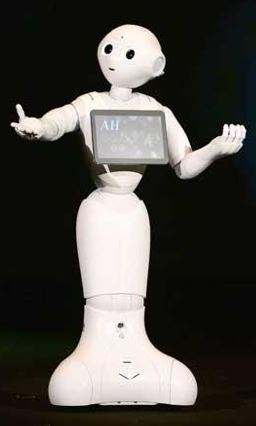
\includegraphics[scale=0.7]{robotPepper}
	\caption{Fotografía del Robot Pepper. \cite{imagen_pepper} }
	\label{fig:RobotPepper}
\end{figure}


Utilizando todas estas herramientas que posee el robot, el problema se puede solucionar de la siguiente manera:

El robot debe estar pendiente de las instrucciones que le indique el paciente, para lo cual, se utilizarán los micrófonos
para grabar el audio (mensaje) emitido por el paciente, posteriormente convertirlo a texto y por último interpretar este
texto como una instrucción. Después de interpretar la instrucción, el robot debe buscar el objeto que le pidió el paciente
mediante el uso de redes neuronales convolucionales de región (en inglés r-cnn: region convolutional neural network).
Si el robot no logra localizarlo, éste deberá notificarle al paciente que no encontró el objeto; por otro lado, si el robot
logra localizar el objeto, éste deberá desplazarse hasta donde está el objeto, sujetar el objeto y llevarlo donde se encuentra
el paciente. El robot debe entregarle el objeto al paciente  en un lugar cercano, por ejemplo, una mesa de noche, con el 
objetivo de velar por la salud y seguridad del paciente. Para términos prácticos el entorno donde se llevará a cabo las 
pruebas y evaluación del proyecto será en el laboratorio de Robótica y Visión Tridimensional en la Universidad de Alicante, España. 
En la figura \ref{fig:DiagramaDeSolucion} se puede brinda un diagrama de flujo que facilita la comprensión de la propuesta para 
hacer frente al problema en cuestión. 



\begin{figure}
	\centering
	\usetikzlibrary{arrows.meta}

\tikzstyle{startstop} = [rectangle, rounded corners, minimum width=3cm, minimum height=1cm,text centered, draw=black, fill=red!30,align=center]

\tikzstyle{io} = [trapezium, trapezium left angle=70, trapezium right angle=110, minimum width=1cm, minimum height=1cm, text centered, draw=black, fill=blue!30,align=center]

\tikzstyle{process} = [rectangle, minimum width=3cm, minimum height=1cm, text centered, draw=black, fill=orange!30,align=center]


\tikzstyle{decision} = [draw, diamond,aspect=2, text centered, draw=black, fill=green!30,inner sep=0pt,align=center]

\tikzstyle{fixedD}=[draw,rectangle split, rectangle split horizontal,align=center,rectangle split parts=3,minimum height=1cm,fill={rgb:red,50;green,200;blue,216}]

\tikzstyle{arrow} = [thick,->,>=stealth]


\newpage
\begin{center}
\begin{tikzpicture}[node distance=1.6cm]

%---------Declaracion de nodos de acción
\node (roslaunch)           [startstop                                                   ] {Inicio Proceso};
\node (espera)              [process , below of=roslaunch                                ] {Estado de espera};
\node (grabar)              [process , below of=espera                                   ] {Grabar audio\\ de instrucción};
\node (traducir)            [process , below of=grabar                                   ] {Traducir audio\\ a texto};
\node (instruccionvalida)   [decision, below of=traducir,node distance=2.3cm             ] {¿Instrucción\\ Valida?};
\node (tomaimagenrgb)       [process , below of=instruccionvalida,node distance=2.3cm    ] {Tomar imagen 2D\\ del entorno};
\node (reconocerobjeto)     [decision, below of=tomaimagenrgb,node distance=2.3cm        ] {¿Objeto\\ Reconocido?};
\node (localizarobjeto)     [process , below of=reconocerobjeto, node distance=2.3cm     ] {Localizar objeto\\ en el entorno};
\node (desplazamiento)      [process , below of=localizarobjeto                          ] {Desplazar el robot hasta el objeto};
\node (tomarobjeto)         [fixedD  , below of=desplazamiento                           ] {\nodepart{two}\shortstack{Tomar objeto\\ con movimientos\\ pregrabados}};
\node (desp_a_paciente)     [process , below of=tomarobjeto                              ] {Desplazar el robot\\ cerca del paciente};
\node (entregarobjeto)      [process , below of=desp_a_paciente                          ] {Entregar el objeto\\ cerca del paciente};
\node (finalizaproceso)     [process , below of=entregarobjeto                           ] {Fin de tarea};


%--------Declaracion de nodos input output
\node (audio)               [io, left of=grabar, xshift=-3cm                             ] {Audio: Mensaje\\ de persona};
\node (imagen2D)            [io, left of=tomaimagenrgb, xshift=-3cm                      ] {Imagen 2D\\ RGB del kinect        };
\node (imagenProfundidad)   [io, left of=localizarobjeto, xshift=-3cm                    ] {Imagen de\\ profundidad\\ del kinect};
\node (inst_no_valida)      [io, right of=instruccionvalida,xshift=4cm                   ] {Respuesta del robot:\\ `Instrucción no valida`};
\node (objeto_no_reconocido)[io, right of=reconocerobjeto,xshift=4cm                     ] {Respuesta del robot:\\ `No se reconoció\\ el objeto`};

%Dibujar flechas de conexion
\draw [arrow] (roslaunch)                  -- (espera);
\draw [arrow] (espera)                     -- (grabar);
\draw [arrow] (grabar)                     -- (traducir);
\draw [arrow] (traducir)                   -- (instruccionvalida);
\draw [arrow] (instruccionvalida)          -- node[anchor=east] {Si}  (tomaimagenrgb);
\draw [arrow] (instruccionvalida)          -- node[anchor=south] {No}  (inst_no_valida);
\draw [arrow] (tomaimagenrgb)              -- (reconocerobjeto);
\draw [arrow] (reconocerobjeto)            -- node[anchor=east] {Si} (localizarobjeto);
\draw [arrow] (reconocerobjeto)            -- node[anchor=south] {No} (objeto_no_reconocido);
\draw [arrow] (localizarobjeto)            -- (desplazamiento); 
\draw [arrow] (desplazamiento)             -- (tomarobjeto);
\draw [arrow] (tomarobjeto)                -- (desp_a_paciente);
\draw [arrow] (desp_a_paciente)            -- (entregarobjeto);
\draw [arrow] (entregarobjeto)             -- (finalizaproceso);
\draw [arrow] (finalizaproceso.west)       -- + (-6,0) |- (espera);
\draw [arrow] (imagen2D)                   -- (tomaimagenrgb);
\draw [arrow] (imagenProfundidad)          -- (localizarobjeto);
\draw [arrow] (audio)                      -- (grabar);
\draw [arrow] (inst_no_valida)             |- (espera);
\draw [arrow] (objeto_no_reconocido.east)  -- + (2,0) |-  (espera);
















\end{tikzpicture}

\end{center}


\newpage
	\caption{Diagrama de Solucion} \label{fig:DiagramaDeSolucion} 
\end{figure}

\newpage





\section{Deep Learning}
agregegar un poco sobre CNN y RPN, luego en marco teorico se amplìa


\section{Datasets}


\section{ROS}



\section{Deep Learning Frameworks}




\section{Metodología utilizada en la investigación}
La metodología utilizada en el proceso de investigación debe ser descrita en forma breve o resumida, de tal manera que el lector comprenda cómo se hizo la tesis y qué elementos fueron utilizados para demostrar o negar la hipótesis (diseño de la investigación, tipo de muestreo empleado, tamaño de la muestra, instrumentos empleados para la recopilación de información, etc.).


\newpage




\section{Objetivos de la investigación}

\begin{enumerate}
    \item{\textbf{Objetivo general:}} 
    
    Diseñar un sistema que asista al paciente en la tarea específica de alcanzar objetos 
    según lo requiera la persona utilizando el robot Pepper
    \item{\textbf{Objetivos específicos}}:
    \begin{enumerate}
    \item Implementar el reconocimiento de los objetos específicos en el entorno que rodea al robot.
        \begin{enumerate}
            \item Indicador: El robot debe reconocer tres objetos pequeños mínimo el 90\% de los intentos 
            en un rango de 1 a 5 metros de distancia.
        \end{enumerate}
    
        \item Implementar el reconocimiento de la voz del paciente y traducirlo como una instrucción.
        \begin{enumerate}
            \item Indicador: El robot debe reconocer la siguientes palabras: traer, alcanzar y los tres nombres 
            de los objetos que se deben reconocer, mínimo un 90\% de los intentos cuando esté a 1 metro de 
            distancia o menos del paciente, una vez que el mensaje haya sido traducido de audio a texto.
        \end{enumerate}
        
        \item Integrar las tareas de desplazamiento y el movimiento de objetos por parte del robot junto con 
        el reconocimiento de objetos y de voz. 
        \begin{enumerate}
            \item Entregable: Esta integración debe cumplir con las métricas definidas anteriormente además 
            de solucionar el problema de la siguiente forma: Cuando la instrucción haya sido interpretada, 
            el robot debe buscar el objeto deseado, determinar su ubicación y desplazarse hasta este a una 
            distancia de aproximadamente 35 centímetros, posteriormente deberá tomarlo y llevarlo hasta una 
            posición cerca del paciente de igual manera a una distancia aproximada de 35 centímetros. 
            Si el robot no logra ubicar el objeto, deberá indicarle al paciente que no logró identificarlo.
            
        \end{enumerate}
    \end{enumerate}
\end{enumerate}




\section{Estructura del documento}
Respecto a la explicación breve del contenido de la investigación se debe narrar en qué consiste cada capítulo 
de la tesis de tal manera que el lector decida continuar leyendo toda la tesis o decida ignorarla por no ser un tema de su interés.

  \chapter{Marco teórico}
\label{ch:marco}






%----OReilly Learning OpenCV.pdf paginas 2-3-----

%\subsection{Visión en Industria automotriz}

%Describirlo muy general




\section{Generalidades}

  %%\chapter{Desarrollo de aplicaciones ADAS basadas en CV y medio de pruebas de control}
\chapter{Casos de estudio bajo funcionamiento exacto}
\label{ch:visioncontrol}

\section{Aplicaciones seleccionadas}

Las selección de las ADAS se hizo luego de realizar la taxonomía. Esto debido a que luego de esa etapa se tenían las bases para escoger. Ante la cantidad de ADAS recopiladas se precisó de un medio de selección para determinar cuales se iban a utilizar para la exploración. Esta selección se basó en 3 puntos:
\begin{itemize}
    \item Disponibilidad inmediata del sensor
    
        Siendo 3 disponible y 0 no disponible
    
    \item Criticidad de no funcionamiento
    
        Siendo 3 muy crítico y 0 nada crítico  
    
    \item Facilidad de implementación
    
        Siendo 3 fácil de implementar y 0 complejo de implementar
\end{itemize}

Se creó una la Tabla 3.1 donde se muestran los valores de cada ADAS según el rubro a evaluar en cada columna y se obtuvo resultados, sumando los valores, en los que particularmente 4 ADAS sobresalieron: TSR, PPS, DSM y LDW. De estas se obtuvo finalmente una lista de las 3. Para simplificarlo se escogieron TSR, PPS y LDW debido a que, de acuerdo a los niveles de autonomía, proporcionan información relevante al vehículo en lo que concierne a su desplazamiento. La DSM si bien es importante debido a su alerta de fatiga no aporta más allá que eso.


\begin{table}[H]
\centering
\caption{Valores para selección}
\label{my-label}
\begin{tabular}{|c|c|c|c|c|}
\hline
ADAS & \begin{tabular}[c]{@{}l@{}}Disponibilidad de \\ sensor utilizado\end{tabular} & \begin{tabular}[c]{@{}l@{}}Criticidad de\\ no funcionamiento\end{tabular} & Implementación & Total \\\hline
TCS  & 2                                                                             & 3                                                                         & 1              & 6     \\
ESC  & 2                                                                             & 3                                                                         & 1              & 6     \\
ACC  & 3                                                                             & 1                                                                         & 2              & 6     \\
ISA  & 1                                                                             & 1                                                                         & 2              & 4     \\
TSR  & 3                                                                             & 3                                                                         & 2              & 8     \\
SLR  & 3                                                                             & 2                                                                         & 2              & 7     \\
AEB  & 2                                                                             & 3                                                                         & 2              & 7     \\
PPS  & 3                                                                             & 3                                                                         & 2              & 8     \\
PCW  & 2                                                                             & 3                                                                         & 1              & 6     \\
CAS  & 2                                                                             & 3                                                                         & 1              & 6     \\
NS   & 2                                                                             & 1                                                                         & 2              & 5     \\
DSM  & 3                                                                             & 3                                                                         & 2              & 8     \\
BSD  & 1                                                                             & 3                                                                         & 2              & 6     \\
LDW  & 3                                                                             & 3                                                                         & 2              & 8     \\
LCA  & 3                                                                             & 2                                                                         & 2              & 7     \\
RVC  & 3                                                                             & 1                                                                         & 3              & 7     \\
IPA  & 2                                                                             & 1                                                                         & 2              & 5     \\
NV   & 1                                                                             & 2                                                                         & 2              & 5     \\
AFS  & 2                                                                             & 2                                                                         & 2              & 6     \\
RSS  & 2                                                                             & 1                                                                         & 3              & 6  \\\hline  
\end{tabular}
\end{table}

Las 3 aplicaciones escogidas son claves para alcanzar ese ansiado nivel 5 de autonomía en la conducción de vehículos.


\subsection{Alerta de Salida del Carril (LDW)}

La detección de carril es fundamental si se desea llegar a ese nivel 5 de autonomía, esto le daría al usuario la tranquilidad de que el vehículo en el que se encuentre va a ser capaz de mantenerse en su carril y no invadir otros, de esta manera accidentes por invasión de carril tanto en el mismo sentido como en sentido contrario de conducción se erradicarían haciendo las calles más seguras.
\newpage
\subsection{Control de Alerta de Peatones (PPS)}

Los peatones si bien no son usuarios propios de las carreteras, pueden estar presentes en ellas. Ya sea por necesidad de cruzar, por que caminan por el espaldón, por la razón que sea no se puede descartar su presencia en las carreteras. Lo que sí se puede hacer es tomar medidas ante la posible aparición de estos en las vías, de esta manera la meta es reducir las estadísticas de atropellos a peatones. 

\subsection{Reconocimiento de Se~nales de Transito (TSR)}

Las señales de transito son indispensables para que el conductor tenga las instrucciones necesarias y delimitar el accionar de estos en las carreteras. Velocidades permitidas, avisos, restricciones, indicaciones de lugares, etc. En este caso nos vamos a enfocar en señales de velocidades permitidas, de este modo indicarle al sistema en que valores de velocidad debe mantenerse según las señalización vertical de las carreteras.

\section{Descripción del capítulo}

El primer caso de estudio comprende en observar el funcionamiento exacto de aplicaciones ADAS, es decir, trabajando tal y como se plantea en los artículos científicos leídos. Se procede a poner en marcha las 3 aplicaciones seleccionadas (TSR, LDW y PCW), todas basadas en CV, para luego probarlas en un sistema de control y obtener una referencia ante que comparar lo que se va a explorar en el siguiente caso de estudio que se presenta en el capítulo 4. Se introducen entonces, los conceptos necesarios para el adecuado entendimiento de lo que este capitulo consiste. 


\subsection*{Visión por Computadora}

La Visión por Computadora (CV), también llamada Visión Artificial, es la transformación de datos de una cámara fotográfica fija o de video en una decisión o una nueva representación. Todas estas transformaciones se hacen para lograr algún objetivo en particular. Los datos de entrada pueden incluir alguna información contextual como "la cámara está montada en un vehículo" o "el láser indica que un objeto está a 1 metro de distancia". La decisión podría ser "hay una persona en esta escena" o "hay 14 células tumorales en esta diapositiva". Una nueva representación puede significar convertir una imagen de color en una imagen en escala de grises o quitar el movimiento de la cámara de una secuencia de imágenes.\cite{Bradski2008}

A pesar de que somos criaturas visuales, es fácil ser engañado en pensar que las tareas de la visión de computadora son fáciles. ¿Qué tan difícil puede ser encontrar un coche cuando lo miras fijamente en una imagen? Sus intuiciones iniciales pueden ser bastante engañosas. El cerebro humano divide la señal de la visión en muchos canales que fluyen diferentes tipos de información en su cerebro. El cerebro tiene un sistema de atención que identifica, de manera dependiente de la tarea, partes importantes de una imagen para examinar mientras se reprime el examen de otras áreas. Hay retroalimentación masiva en el flujo visual que es, hasta ahora, poco entendido. Existen insumos asociativos generalizados de los sensores de control muscular y de todos los otros sentidos que permiten al cerebro dibujar en asociaciones cruzadas hechas a partir de años de vida en el mundo. Los bucles de retroalimentación en el cerebro se remontan a todas las etapas de procesamiento, incluyendo los propios sensores de hardware (los ojos), que controlan mecánicamente la iluminación a través del iris y afinan la recepción en la superficie de la retina. La visión de la computadora es un campo que crece rápidamente, en parte como resultado de cámaras más baratas y más capaces, en parte debido a la energía de proceso comprable, y en parte porque los algoritmos de la visión están comenzando a madurar. OpenCV en sí ha desempeñado un papel en el crecimiento de la visión de la computadora al permitir que miles de personas hagan un trabajo más productivo en la visión. Con su enfoque en la visión en tiempo real, OpenCV ayuda a los estudiantes y profesionales a implementar eficientemente proyectos y a iniciar la investigación, proporcionándoles una visión de la computadora y la infraestructura de aprendizaje de máquinas que anteriormente estaba disponible sólo en unos pocos laboratorios de investigación madura.\cite{Bradski2008}

\subsection*{Control Automático}

En esta sección se pretende dar una visión general de lo que el Control Automático significa y para ello se comienza con una serie de conceptos básicos recopilados de \cite{Ogata2013} los cuales se exponen a continuación:

La \textbf{variable controlada} es la cantidad o condición que se mide y controla. 
La \textbf{señal de control} es la cantidad o condición que el controlador modifica para afectar el valor de la variable controlada.

\textbf{Controlar} significa medir el valor de la variable controlada del sistema y aplicar la variable manipulada al sistema para corregir o limitar la desviación del valor medido respecto del valor deseado. En el estudio de la ingeniería de control, es necesario definir términos adicionales que se precisan para describir los sistemas de control.

Una \textbf{planta} puede ser una parte de un equipo, tal vez un conjunto de los elementos de una máquina que funcionan juntos, y cuyo objetivo es efectuar una operación particular. En este libro se llamará planta a cualquier objeto físico que se va a controlar (como un dispositivo mecánico, un horno de calefacción, un reactor químico o una nave espacial).

El Diccionario Merriam-Webster define un \textbf{proceso} como una operación o un
desarrollo natural progresivamente continuo, marcado por una serie de cambios graduales que se suceden unos a otros de una forma relativamente fija y que conducen a un resultado o propósito determinados; o una operación artificial o voluntaria que se hace de forma progresiva y que consta de una serie de acciones o movimientos controlados, sistemáticamente dirigidos hacia un resultado o propósito determinado. En este libro se llamará proceso a cualquier operación que se va a controlar. Algunos ejemplos son los procesos químicos, económicos y biológicos.

Un \textbf{sistema} es una combinación de componentes que actúan juntos y realizan un objetivo determinado. Un sistema no está necesariamente limitado a los sistemas físicos. El concepto de sistema se puede aplicar a fenómenos abstractos y dinámicos, como los que se encuentran en la economía. Por tanto, la palabra sistema debe interpretarse en un sentido amplio que comprenda sistemas físicos, biológicos, económicos y similares.

Una \textbf{perturbación}  es una señal que tiende a afectar negativamente el valor de la salida de un sistema. Si la perturbación se genera dentro del sistema se denomina interna, mientras que una perturbación externa se genera fuera del sistema y es una entrada.

El \textbf{control realimentado} se refiere a una operación que, en presencia de perturbaciones, tiende a reducir la diferencia entre la salida de un sistema y alguna entrada de referencia, y lo realiza tomando en cuenta esta diferencia. Aquí sólo se especifican con este término las perturbaciones impredecibles, ya que las perturbaciones predecibles o conocidas siempre pueden compensarse dentro del sistema

\subsection*{Tipos de Controladores}
\subsubsection*{Lazo Cerrado vs Lazo Abierto}

Sistemas de control en lazo cerrado en comparación con sistemas en lazo abierto. Una ventaja del sistema de control en lazo cerrado es que el uso de la realimentación vuelve la respuesta del sistema relativamente insensible a las perturbaciones externas y a las variaciones internas en los parámetros del sistema. Es así posible usar componentes relativamente poco precisos y baratos para obtener el control adecuado de una planta determinada, mientras que hacer eso es imposible en el caso de un sistema en lazo abierto. Desde el punto de vista de estabilidad, el sistema de control en lazo abierto es más fácil de desarrollar, porque la estabilidad del sistema no es un problema importante. Por otra parte, la estabilidad es un gran problema en el sistema de control en lazo cerrado, que puede conducir a corregir en exceso errores que producen oscilaciones de amplitud constante o cambiante. Debe señalarse que, para los sistemas en los que se conocen con anticipación las entradas y en los cuales no hay perturbaciones, es aconsejable emplear un control en lazo abierto. Los sistemas de control en lazo cerrado sólo tienen ventajas cuando se presentan perturbaciones y/o variaciones impredecibles en los componentes del sistema. El número de componentes usados en un sistema de control en lazo cerrado es mayor que el que se emplea para un sistema de control equivalente en lazo abierto. Por tanto, el sistema de control en lazo cerrado suele tener costes y potencias más grandes. Para disminuir la potencia requerida de sistema, se emplea un control en lazo abierto siempre que pueda aplicarse. Por lo general, una combinación adecuada de controles en lazo abierto y en lazo cerrado es menos costosa y ofrecerá un comportamiento satisfactorio del sistema global.
En ciertas circunstancias (por ejemplo, si no hay perturbaciones o la salida es difícil de medir) pueden ser deseables los sistemas de control en lazo abierto. Por tanto, es conveniente resumir las ventajas y desventajas de utilizar sistemas de control en lazo abierto\cite{Ogata2013}

\subsubsection*{Controlador P }

La acción de control proporcional, da una salida del controlador que es proporcional al error y puede
controlar cualquier planta estable, pero posee desempeño limitado y error en régimen permanente\cite{Mazzone2012}.

\subsubsection*{Controlador I }

Da una salida del controlador que es proporcional al error acumulado, lo que implica que es un modo de controlar lento\cite{Mazzone2012}.

\subsubsection*{Controlador PI }

Con un control proporcional, es necesario que exista error para tener una acción de control distinta de cero. Con acción integral, un error pequeño positivo siempre nos dará una acción de control creciente, y si fuera negativo la señal de control ser a decreciente. Este razonamiento sencillo nos muestra que el error en régimen permanente sera siempre cero. Muchos controladores industriales tienen solo acción PI. Se puede demostrar que un control PI es adecuado para todos los procesos donde la dinámica es esencialmente de primer orden\cite{Mazzone2012}.

\subsubsection*{Controlador PD }

Esta acción tiene carácter de previsión, lo que hace más rápida la acción de control, aunque tiene la desventaja importante que amplifica las señales de ruido y puede provocar saturación en el actuador. La acción de control derivativa nunca se utiliza por sí sola, debido a que solo es eficaz durante perıodos transitorios. Cuando una acción de control derivativa se agrega a un controlador proporcional, permite obtener un controlador de alta sensibilidad, es decir que responde a la velocidad del cambio del error y produce una corrección significativa antes de que la magnitud del error se vuelva demasiado grande.

\subsubsection*{Controlador PID }

Esta acción combinada reúne las ventajas de cada una de las tres acciones de control individuales\cite{Mazzone2012}.
\newpage


\section{Visión por Computadora}

Las aplicaciones ADAS seleccionadas, se desarrollan y adaptan para obtener resultados que, en una primera versión, son aceptables y muestran de manera general lo que se quiere realizar en cada una de ellas en su versión final. Mediante programación en c++ y las librerías y funciones específicas de OpenCV se logró obtener resultados provisionales del avance hasta el día de la presentación de este avance.


\subsection{Resultados para primer avance}
\subsubsection{LDW}

Lo obtenido al programar la LDW es lo que se presenta en la Figura 3.1. En la fila superior se muestra con lineas finas amarillas la Región de Interés (ROI) que es zona que se quiere estudiar, de esta manera solo procese esta y no la totalidad de la imagen, esto a manera de preprocesamiento. Seguidamente se genera una vista "Bird Eye" o vista de pájaro a partir de la ROI seleccionada anteriormente de este modo ya se cuenta con un panorama más claro y sencillo de estudiar. A este se le detectan bordes y se trazan lineas sobre ellos y se obtiene así la vista que se encuentra en la esquina superior derecha de la Figura 3.1. Finalmente se le realiza reacomoda en la imagen original se logra observar en la vista inferior de la Figura 3.1 que las indicaciones rojas calzan sobre las lineas. En dicha figura se muestra un cuadro del video completo, pero la aplicación corre sobre una grabación de un vehículo andando. Se puede observar un video de esta primera versión en: \url{https://youtu.be/myVD5Tk01nE}

\begin{figure}[H]
  \centering
  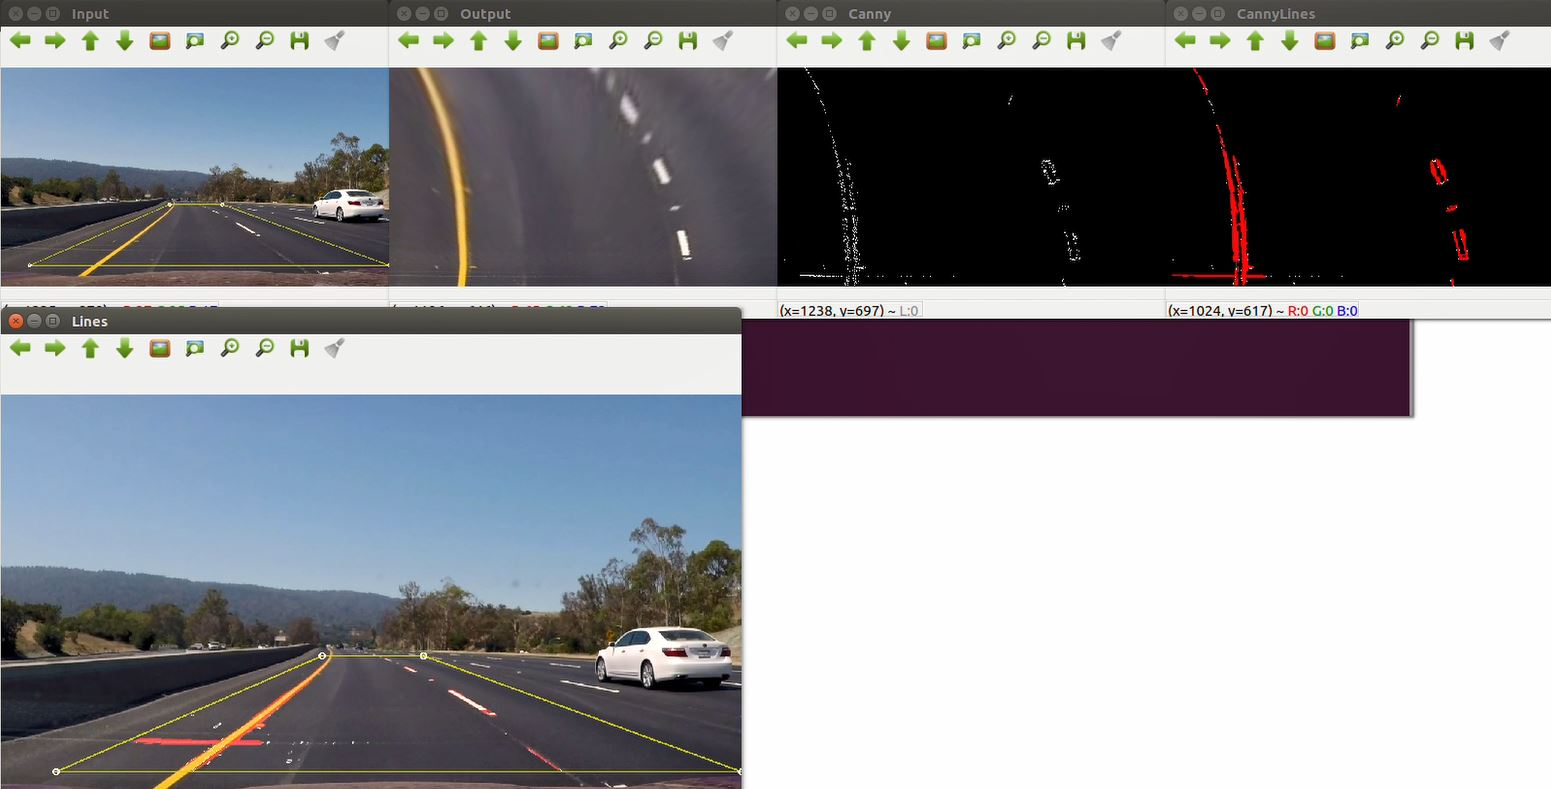
\includegraphics[width=0.9\textwidth]{ldw.JPG}
  \caption{Primeros resultados LDW}
  \label{fig:boat2}
\end{figure}


\begin{figure}[H]
  \centering
      \begin{tikzpicture}[node distance = 1.5cm, auto]
        % Place nodes
        \node [block] (init) {inicio};
        \node [block, below of=init] (prepro) {pre-procesamiento y demarcación de ROI};
        \node [block, below of=prepro] (detect) {detectar ROI};
        \node [block, below of=detect] (bird) {transformacion vista de pájaro};
        \node [block, below of=bird] (canny) {detectar bordes};
        \node [block, below of=canny] (lines) {trazar líneas};
        \node [decision, below of=lines] (decide) {¿Está centrado?};
        \node [block, below of=decide, node distance=3cm] (stop) {Emita alerta};
        \node [block, right of=canny, node distance=5cm] (update) {siguiente cuadro};
        % Draw edges
        \path [line] (init) -- (prepro);
        \path [line] (prepro) -- (detect);
        \path [line] (detect) -- (bird);
        \path [line] (bird) -- (canny);
        \path [line] (canny) -- (lines);
        \path [line] (lines) -- (decide);
        \path [line] (decide) -- node {si}(stop);
        \path [line,dashed] (stop) -| (update);
        \path [line] (decide) -| node [near start] {no}(update);
        \path [line,dashed] (update) |- (detect);
    \end{tikzpicture}    
  \caption{Diagrama flujo LDW propuesta}
  \label{fig:diag_ldw}
\end{figure}

\newpage


\subsubsection{PPS}

El detector de peatones se presenta en la Figura 3.2. En ella se observan 4 vistas de los pasos que se iban realizando para la obtención del resultado deseado. Los 2 cuadros del centro de la figura son pasos de preprocesamiento para finalmente poder aplicar una herramienta de detección de personas mediante cascada. Se puede observar un par de videos de esta primera versión en: \url{https://youtu.be/Rxt\_fKXrZTA} y en \url{https://youtu.be/pQZbL1H1IKk}

\begin{figure}[H]
  \centering
    \begin{tikzpicture}[node distance = 1.5cm, auto]
        % Place nodes
        \node [block] (init) {inicio};
        \node [block, below of=init] (prepro) {pre-procesamiento y demarcación de ROI};
        \node [block, below of=prepro] (roi1) {detectar peatón};
        \node [decision, below of=roi1] (decide) {¿Peatón en ROI?};
        \node [block, below of=decide, node distance=2.5cm] (stop) {Emita alerta};
        \node [block, right of=roi1, node distance=6cm] (update) {siguiente cuadro};
        % Draw edges
        \path [line] (init) -- (prepro);
        \path [line] (prepro) -- (detect);
        \path [line] (detect) -- (roi1);
        \path [line] (roi1) -- (decide);
        \path [line] (decide) -- node {si}(stop);
        \path [line,dashed] (stop) -| (update);
        \path [line] (decide) -| node [near start] {no}(update);
        \path [line,dashed] (update) -- (roi1);
    \end{tikzpicture}    
  \caption{Diagrama flujo PPS propuesta}
  \label{fig:diag_pps}
\end{figure}

\begin{figure}[H]
  \centering
  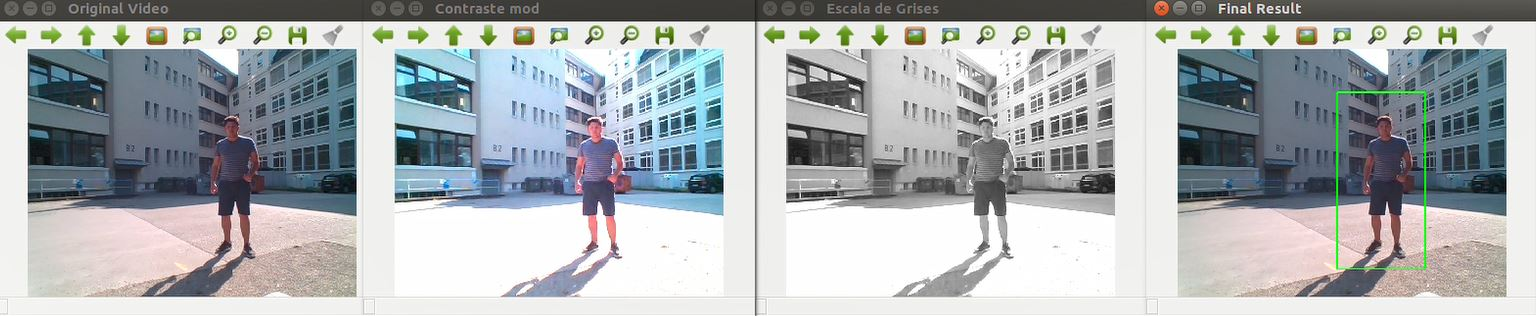
\includegraphics[width=0.8\textwidth]{pcw.JPG}
  \caption{Primeros resultados PPS }
  \label{fig:boat2}
\end{figure}
\newpage

\subsubsection{TSR}
El detector de señales de tránsito actualmente está en desarrollo. Del video fuente se detecta mediante cascada la zona que se desea analizar. Esta zona se asigna como ROI y se despliega en una ventana aparte. Al centro abajo de la Figura 3.3 se muestra una imagen que funciona como referencia ante que comparar la ROI seleccionada. Se pretende mediante comparación de histogramas determinar si la ROI es igual o compatible con la imagen de referencia. Para no meter ruido al histograma se debe generar otra ROI donde se elimine el anillo oscuro alrededor del número de la señal detectada. Se puede observar un de video de esta primera versión en: \url{https://youtu.be/Ku82Fxoz5P0}


\begin{figure}[H]
  \centering
    \begin{tikzpicture}[node distance = 1.5cm, auto]
        % Place nodes
        \node [block] (init) {inicio};
        \node [block, below of=init] (prepro) {pre-procesamiento};
        \node [block, below of=prepro] (detect) {detectar señal};
        \node [block, below of=detect] (roi1) {demarcar la señal como ROI};
        \node [block, below of=roi1] (roi2) {demarcar los dígitos con una ROI};
        \node [decision, below of=roi2] (decide) {¿Nuevo límite?};
        \node [block, below of=decide, node distance=2.25cm] (stop) {Despliegue valor de velocidad};
        \node [block, right of=roi2, node distance=5cm] (update) {siguiente cuadro};
        % Draw edges
        \path [line] (init) -- (prepro);
        \path [line] (prepro) -- (detect);
        \path [line] (detect) -- (roi1);
        \path [line] (roi1) -- (roi2);
        \path [line] (roi2) -- (decide);
        \path [line] (decide) -- node {si}(stop);
        \path [line,dashed] (stop) -| (update);
        \path [line] (decide) -| node [near start]{no}(update);
        \path [line,dashed] (update) |- (detect);
    \end{tikzpicture}    
  \caption{Diagrama flujo TRS propuesta}
  \label{fig:diag_tsr}
\end{figure}


\begin{figure}[H]
  \centering
  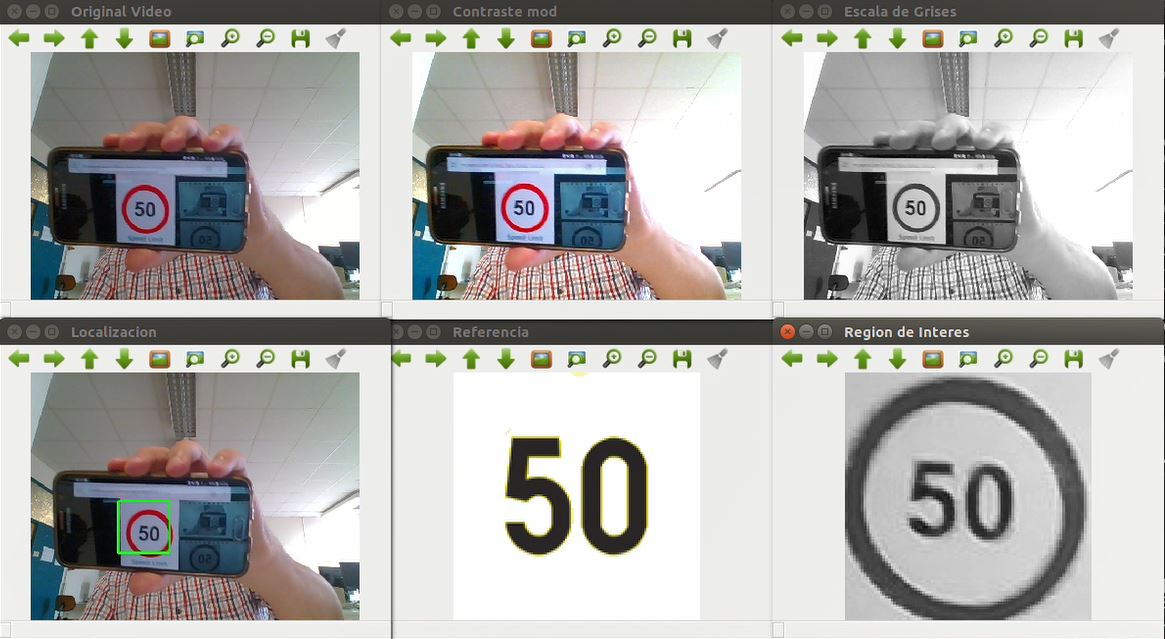
\includegraphics[width=0.45\textwidth]{tsr.JPG}
  \caption{Primeros resultados TSR}
  \label{fig:results_trs}
\end{figure}
  %\chapter{Casos de estudio bajo funcionamiento aproximado}
\label{ch:aproximado}

\section{Descripción del capítulo}

Este segundo caso de estudio comprende en observar el funcionamiento aproximado de aplicaciones ADAS. Se procede realizar modificaciones a las 3 aplicaciones seleccionadas (TSR, LDW y PCW), para luego probarlas en un sistema de control y obtener data que comparar contra lo que se va a obtuvo en el caso de estudio que se presentó en el capítulo 3. Se introducen entonces, los conceptos necesarios para el adecuado entendimiento de lo que este capitulo consiste. 

\subsection*{Paradigmas de diseño en computación}

A pesar de los avances en tecnologías de semiconductor y desarrollo de técnicas del diseño eficientes por la energía, el consumo de energía total de sistemas de ordenadores todavía crece rápidamente en un ritmo alarmante a fin de tratar una cantidad creciente de la información. En particular, ya que los sistemas de ordenadores se hacen penetrantes, cada vez más son usados para relacionarse con el mundo físico y tratar una cantidad grande de datos de varias fuentes. Además, esperamos que ellos sean el contexto consciente y presenten interfaces de usuario naturales. Por consiguiente, un gran número de aplicaciones, comúnmente referidas como el reconocimiento, minería, y síntesis (Recognition, Mining, and Synthesis, RMS) aplicaciones, ha surgido y explican una parte significativa de recursos computacionales a través del espectro de calcular, desde móvil y dispositivos de Internet of Things (IoT) a centros de datos a gran escala.
Es esencial mejorar dramáticamente la eficiencia energética de estas cargas de trabajo emergentes a fin de mantener el ritmo del crecimiento de la información que necesita ser procesada. Afortunadamente, estas aplicaciones suelen presentar una propiedad intrínseca de la resiliencia de errores [2]. Procesan datos ruidosos y redundantes de fuentes de entrada no tradicionales como varios tipos de sensores (entradas inexactas) y los algoritmos asociados son a menudo estocásticos en la naturaleza (por ejemplo, algoritmos iterativos)\cite{Xu2016}.



\subsection*{Computación Aproximada}

La computación aproximada, ha atraído la tracción significativa tanto de academia como de industria. Relajando la equivalencia numérica entre la especificación y la realización de aplicaciones tolerantes del error, la informática aproximada deliberadamente introduce errores aceptables [en el proceso de calcular y promete ganancias de eficiencia energética significativas. La consideración del hecho que el escalamiento de Dennard tradicional provee rendimientos decrecientes del progreso de la tecnología, reforzando la nueva fuente de eficiencia energética proporcionada por la informática aproximada es cada vez más importante\cite{Xu2016}.

\subsubsection*{Software Aproximado}

Un buen lenguaje de programación debería permitir a los programadores para ser productivos. Se debe permitir a los programadores rápidamente expresar sus ideas como programas y al mismo tiempo permitir un compilador o un sistema de ejecución para optimizar sus programas de ejecución. En muchos sentidos, un lenguaje de programación y su aplicación equilibrar la productividad de los programadores con un sistema s eficiencia. El mecanismo por el cual los lenguajes de programación proporcionan este equilibrio es la abstracción. Una abstracción permite al programador a decir qué hacer con el fin de realizar una tarea, no cómo hacerlo. La forma de hacerlo o la aplicación de la abstracción es la izquierda para el compilador o el sistema de ejecución. Construcción de aplicaciones sofisticadas, es difícil y requiere experiencia en toda la pila del sistema, y en esta época de aproximación, que experiencia incluye estadísticas (o alguna otra aproximación consciente razonamiento) además de aplicación el conocimiento de dominios específicos. No es de extrañar, entonces, que muchos investigadores hayan propuesto abstracciones para ayudar a los programadores con esta tarea desalentadora. Estas abstracciones ayudan a los programadores a expresar sus ideas en código (es decir, lenguajes de programación con conciencia aproximada), permita que los motores de análisis razonen sobre la corrección de tales programas (es decir, análisis aproximados), y permita que los compiladores generen código de máquina (es decir, compiladores con conciencia aproximada). Esta sección revisa el trabajo académico e industrial reciente de estas áreas de lenguajes de programación orientados al aproximado, análisis aproximados y compiladores con conciencia aproximada\cite{Xu2016}.


%------Aproximate Computing:A survey----survey.pdf---------------

%%%%%%%%%%%%%%%%%%%%%%%%%%%%%%%%%%%%%%%%%%%%%%%%%%%%%%%%%%%%%%%%%%%%%%%%%%%%%%%%%%%%%%


\begin{comment}
Primero que todo, jamás utilice el título indicado arriba, sino algo
relacionado con su solución: ``Sistema de corrección de distorsión'' o lo que
competa a su tesis en particular.

Este capítulo puede separarse en varias secciones, dependiendo del problema
concreto. Aquí los algoritmos o el diseño del sistema deben quedar lo
suficientemente claros para que otra persona pueda re-implementar al sistema
propuesto. Sin embargo, el enfoque no debe nunca concentrarse en los detalles
de la implementación particular realizada, sino del diseño conceptual como tal.

Recuerdese que toda figura y tabla deben estar referenciadas en el texto.
\end{comment}
  \chapter{Integracion de tareas }
\label{ch:solucion}




\section*{Procedimiento para la ejecución del proyecto}

Este proyecto reúne distintas disciplinas como visión artificial (computer vision), aprendizaje profundo 
(deep learning), integración de tareas mediante software tipo middleware (lógica de intercambio de información
entre aplicaciones), nubes de puntos, entre otros. A continuación se explica las actividades que se pretenden 
aplicar para lograr cada etapa planteada en los objetivos específicos.


\section{Reconocer los objetos especificados en el entorno que rodea al robot:}
Se deben hacer diferentes pruebas
para definir los parámetros y condiciones óptimas para realizar la captura de las imágenes. Después se utilizará
Caffe (framework) el cual soporta muchos tipos diferentes de arquitecturas de aprendizaje profundo, en este caso
se utilizará el proyecto \textit{Faster R-CNN: Towards Real-Time Object Detection with Region Proposal Networks}
\cite{renNIPS15fasterrcnn}, orientada a la clasificación de objetos en imágenes y la ubicación de la región donde
se encuentre. Se utilizarán modelos de redes neuronales convolucionales pre-entrenados que se fundamenten en la
base de datos ImageNet la cual está organizada de acuerdo a la jerarquía de sustantivos de WordNet en el que cada
nodo de la jerarquía está representado por cientos y miles de imágenes, aunque también en caso de ser necesario 
se entrenará una red neuronal con un \textit{dataset} enfocado en reconocer específicamente los objetos previamente 
detallados para obtener un modelo que presente mayores beneficios en comparación a los ya existentes. Los objetos 
específicos que debe reconocer el robot aún están por definir porque la mano en el brazo del robot no es muy grande
y se deben hacer pruebas con objetos pequeños para definirlos. En pocas palabras, Caffe se encarga de recibir como
\textbf{entrada} una imagen tomada por el robot y su \textbf{salida} es o son los sustantivos u objetos que más 
probabilidad tienen de coincidir con la realidad junto con la ubicación de la región donde reconoció el objeto. 
 
\section{Reconocer la voz del paciente y traducirlo como una instrucción:}
El reconocimiento de voz se llevará a cabo
mediante bibliotecas que se importan en Python para cumplir este objetivo. Por ejemplo, el primer candidato para 
esta tarea es SpeechRecognition la cual es una biblioteca para Python soportado por la API Google Speech Recognition.
Este tiene la función de convertir el mensaje del paciente a texto, y posteriormente el robot deberá interpretarlo
como una instrucción. Se debe aclarar que después de la conversión de audio a texto, el algoritmo atenderá a
instrucciones y objetos limitados, con el objetivo de simplificar el proyecto debido al corto periodo para 
desarrollarlo. Las palabras que debe reconocer según las métricas definidas son: 
    \begin{itemize}
        \item Verbos: Traer, alcanzar.
        \item Sustantivos: Los tres nombres de los objetos que se deben localizar
    \end{itemize}
    
    
\section{ Integrar las tareas de desplazamiento y el movimiento de objetos por parte del robot junto con 
    el reconocimiento de objetos y de voz: }
Para lograr la localización en el espacio del robot y el objeto 
deseado se hará uso del dispositivo tipo Kinect o sensor 3D para obtener información del entorno que rodea
al robot y luego procesarla con PCL (Point Cloud Library) la cual incorpora utilidades para trabajar con
nubes de puntos y procesamiento de imágenes 3D, esto tiene como finalidad de que el robot se ubique en el 
espacio que lo rodea pero también sirve para identificar dónde se encuentra el objeto deseado. Luego que se 
ha localizado el objeto, el robot debe desplazarse hasta las cercanías de este, tomar el objeto mediante un 
movimiento pregrabado (con el fin de evitar la ardua tarea de \textit{Grasping} en robótica), regresar hasta 
donde se encuentra el paciente y colocarlo cerca según las especificaciones previamente definidas.
    
Para obtener toda esta información de los sensores del robot y también para accionar sus motores que permiten
desplazarlo entre distintos puntos y mover sus extremidades se utilizará el sistema operativo para robots que
se caracteriza por ser un software de tipo middleware (ROS: Robot Operating System), el cual opera de la 
siguiente manera: el núcleo donde se realiza todo el procesamiento de la información es el ordenador, el 
cual se conecta al robot que en este caso es una ramificación del núcleo mediante su IP dentro de una red,
de esta manera el núcleo puede acceder a todos los dispositivos del robot como cámara, sensores, kinect,
micrófonos y también puede accionar los mecanismos para mover al robot y sus extremidades.
    
Algunos puntos a considerar:
    \begin{itemize}
        \item Delimitar la altura en la que se encuentra el objeto, la cual ronda un rango entre 70 cm a 100 cm
        \item La mano del robot o pinza se abrirá y cerrará en dirección paralela al suelo.
        \item El proyecto no tiene como requisito contemplar obstáculos.
        \item Este proyecto no tiene como requisito que su evaluación sea en un entorno real como un cuarto 
        de habitación, un cuarto de hospital, entre otros; esto por el corto periodo para desarrollar el proyecto. 
    \end{itemize}
 
Por último se debe lograr enlazar cada tarea individual y crear un sistema funcional, en esta etapa 
es posible que se deban hacer modificaciones a las tareas individuales para mejorar los resultados del proyecto.  
    


  %\chapter{Resultados y análisis}

\begin{comment}
En tesis formales en este capítulo se exponen los diseños experimentales
realizados para comprobar el funcionamiento correcto del sistema. Por ejemplo,
si se realiza algún sistema con reconocimiento de patrones, usualmente esta
sección involucra las llamadas \emph{matrices de confusión} donde se compactan
las estadísticas de reconocimiento alcanzadas. En circuitos de hardware,
experimentos para determinar variaciones contra ruido, etc. También pueden
ilustrarse algunos resultados concretos como ejemplo del funcionamiento de los
algoritmos. Puede mostrar por medio de experimentos ventajas, desventajas,
desempeño de su algoritmo, o comparaciones con otros algoritmos.

Recuerde que debe minimizar los ``saltos'' que el lector deba hacer en su
documento. Por tanto, usualmente el análisis se coloca junto a tablas y figuras
presentadas, y debe tener un orden de tal modo que se observe cómo los
objetivos específicos y el objetivo general del proyecto se han cumplido.
\end{comment}

%Exponer que se va a realizar

\section{Resultados}

\subsection{Visión Exacta}

Resultados obtenidos de los programas desarrollados 

\subsubsection{ADAS 1}

\subsubsection{ADAS 2}

\subsubsection{ADAS 3}


\subsection{Visión Aprox}

Resultados obtenidos de los programas desarrollados con algoritmos de aproximación implementados


\subsubsection{ADAS 1}

\subsubsection{ADAS 2}

\subsubsection{ADAS 3}

\subsection{Control Exacta}

Resultados obtenidos del sistema de control bajo funcionamiento exacto

\subsubsection{ADAS 1}

\subsubsection{ADAS 2}

\subsubsection{ADAS 3}


\subsection{Control Aprox}

Resultados obtenidos del sistema de control bajo funcionamiento Aproximado

\subsubsection{ADAS 1}

\subsubsection{ADAS 2}

\subsubsection{ADAS 3}


\section{Análisis}

\subsection{Visión Exacta}

\subsection{Visión Aprox}

\subsection{Visión Exacta vs. Aprox}

\subsection{Control Exacta}

\subsection{Control Aproximada}

\subsection{Control Exacta vs. Aprox}
  %\chapter{Conclusiones}

\begin{comment}Las conclusiones no son un resumen de lo realizado sino a lo que ha llevado el
desarrollo del proyecto, no perdiendo de vista los objetivos planteados desde
el principio y los resultados obtenidos.  En otras palabras, qué se concluye o
a qué se ha llegado después de realizado el proyecto de graduación.  Un error
común es ``concluir'' aspectos que no se desarrollaron en la tesis, como
observaciones o afirmaciones derivadas de la teoría directamente.  Esto último
debe evitarse.

Es usual concluir con lo que queda por hacer, o sugerencias para mejorar los
resultados.

\end{comment}

  %----------------------------------------------------------------------------
  % literature
  \bibliographystyle{IEEEtran} % for english documents
  \bibliography{refe}
  %----------------------------------------------------------------------------

  %----------------------------------------------------------------------------
%  \appendix
  %----------------------------------------------------------------------------

%  \chapter{Primer Apendice}




codigos fuentes

manuales

etc

etc

etc




  %----------------------------------------------------------------------------
  \backmatter
  %----------------------------------------------------------------------------

%  \printindex                % insert index into document. Don't forget to call
                             % "makeindex filename" first.
\end{document}
